\documentclass[UTF8]{ctexart}
    \title{\huge Code Reading Report V2}
    \author{\large 2015011308 唐适之}
    \date{}
    \usepackage[top=1in, bottom=1in, left=1.25in, right=1.25in]{geometry}
    \usepackage{enumitem}
	\usepackage{graphicx}
    \renewcommand{\figurename}{Figure}
    \renewcommand{\contentsname}{Contents}

\begin{document}
    
    \maketitle

    \tableofcontents

    \section{Introduction}

        This report describes the architecture and system design of \textit{LiquidFun}, including its components, workflow, advanced techniques, and key design principles. This is not a API reference, and will not cover all the detailed functions.

        \textit{LiquidFun} is a 2D rigid-body and fluid simulation C++ library for games based upon \textit{Box2D}. It provides support for procedural animation of physical bodies to make objects move and interact in realistic ways\footnote{http://google.github.io/liquidfun/ Overview}. It brings particles to \textit{Box2D} so as to simulate fluid. \textit{LiquidFun} is not a physical simulator for scientific analysing. It provides an approximate but efficient way of calculation. \textit{LiquidFun} is either not a game framework. It only provides an interface to calculate the physics, but does not involves in displaying and controling.

    \section{Building}
        
        The official \textit{LiquidFun Build and Run Instructinos} gives a specific building guide on different platforms. Here is a brief repeat on how to build it on a Linux, as well as something that is not mentioned in the official guide.

        \subsection{Dependencies}

            The official guide gives 3 minimum dependencies:
            
            \begin{itemize}
                \item OpenGL: libglapi-mesa 8.0.4
                \item GLU: libglu1-mesa-dev 8.0.4
                \item cmake: 2.8.12.1
            \end{itemize}

            In a Debian origined Linux, like Ubuntu, they can be installed as below:

            \begin{itemize}
                \item sudo apt-get install cmake
                \item sudo apt-get install libglapi-mesa
                \item sudo apt-get install libglu1-mesa-dev
            \end{itemize}

            There might be two missing dependencies: \textit{X11 client-side library (Xlib)}, which provides an API to the basic X Window System, and \textit{X11 Input extension library (libXi)}, which provides an API to the XINPUT extension to the X protocol. In a Ubuntu system, it can be installed via \textit{sudo apt-get install libx11-dev libxi-dev}. If compiling without them, the compiler will report that it cannot find \textit{X11/Xlib.h} or \textit{X11/extensions/XInput2.h} especially.

        \subsection{Compiling}

            As described in the guide, we use \textit{cmake} to compile the project as below.

            \begin{itemize}
                \item \textit{cd liquidfun/Box2D} \# switch to the corresponding directory
                \item \textit{cmake -G'Unix Makefiles'} \# generate Makefile using cmake
                \item \textit{make}
            \end{itemize}

            In the ideal case, it should have been done, but there is a known issue in the CMakeLists.txt, which is used by cmake, even in the stable version. The CMakeLists.txt should have load the \textit{Thread} package to load a multithread library for the corresponding platform, but the loading instruction is simply missing for some platforms however. In this situation, try adding \textit{find\_package(Threads)} in the CMakeLists.txt. This rough patch may not work for every platform because the instruction might not needed on some platform, but it should resolve the issue when the problem truly occurs.

        \subsection{Run to test}

            Under a full building, to determine whether we have complete a successful building, execute
            
            \textit{./liquidfun/Box2D/Testbed/Release/Testbed}
            
            \noindent to run a demo, or execute
            
            \textit{./liquidfun/Box2D/Unittests/run\_tests.sh}
            
            \noindent to run unit tests.

    \section{Usage}

        \textit{LiquidFun} is a library to calculate 2D rigid body and liquid physics, extended from \textit{Box2D}. It just does the math, but does not include the displaying function. We have to implement our own programs that makes use of \textit{LiquidFun}.
        
        \subsection{Using the Framework and Linking the Libraries}

            Under a full building, the following parts will be built to their respective directives. (On a Linux platform)

            \begin{itemize}
                \item \textit{Box2D}. It's \textit{LiquidFun} itself, the core library. Modules below are not necessarily part of \textit{LiquidFun}.
                \item \textit{HelloWorld}. A minimum demo consisting no GUI, just displying the calculated digits.
                \item \textit{freeglut} and \textit{glui}. They are APIs to access OpenGL (a 3D graph library) easily, providing a basic UI library. They help to build a program that can display the result on screen as it is.
                \item \textit{Testbed}. It's a demo or a UI program built to display the result, making use of \textit{freeglut} and \textit{glui}, so when we are working with \textit{LiquidFun}, it's no need to implement the display program by ourselves, even we have \textit{freeglut} or \textit{glui}. As the name indicates, \textit{Testbed} can also help do some debugging, such as printing debug info or doing step-by-step executing.
                \item \textit{googletest}. It's a framework that help building unit tests.
                \item \textit{Unittests}. Unit tests for \textit{LiquidFun}.
            \end{itemize}
            
            If we tend to ignore the GUI, or to implement the UI by ourselves, we only need to include the headers and link the libraries in \textit{Box2D} directive, Or we can put our code in the \textit{Testbed} and compile it together with the \textit{Testbed}.

        \subsection{Run the Physics World}

            To make a brief explaination, there are roughly three steps to run the \textit{LiquidFun}:

            \begin{itemize}
                \item Create a World. A \textit{b2World} object handles all infrastructural work, including memory allocating and objects management, so we should create a \textit{b2World} object first before adding objects to it.
                \item Adding Objects. Several objects shold be added to \textit{b2World}, including \textit{b2Body}(s), which act as priticles, \textit{b2Fixture}(s), which give \textit{b2Body} shape and physical parameters, and other additional objects.
                \item Call \textit{b2World::Step} to simulate the physics step by step with a discret time interval. Between each simulation, we can get access to the objects to get their parameters or make operations on them.
            \end{itemize}

            More details can be referred to the document and is no need to be repeated here.

    \section{System Overview}

        Sections below are only about the core parts of \textit{LiquidFun}, but not involved with extensions such as \textit{Testbed}.

        There are three major modules inherited from \textit{Box2D}: Common, Collision and Dynamics. The Common module is an infrastructure, which provides memory allocation, math, settings and data structures. The Collision module takes charge of static geometry, which defines shapes and handles geometric queries. The Dynamics module simulates the physics using the two module above.

        The Dynamics module can only do with rigid bodies, and therefore a Particle moudle is added in \textit{LiquidFun}, which provides simulation of particles. There is also a Rope module which seems to be uncompleted however.

        The figure below is the relations among these modles, extended from the graph in \textit{Box2D} document, which describes the three \textit{Box2D} modules. In this figure, the modules below make use of the modules above.

        \begin{figure}[ht]
            \centering
            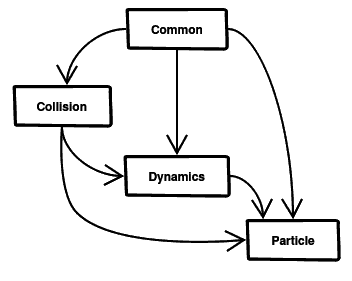
\includegraphics[width=.5\textwidth]{modules.png}
            \caption{Modules}
        \end{figure}

    \section{OOP Design}

        \subsection{Factories}

            Classes like \textit{b2Body}, \textit{b2Fixture} are created by factory functions but not directly by constructors. Because these classes should bind to a parent class to play its role, their factory class is just their parent class. For example, class \textit{b2Body} has a member function
            
            \textit{b2Fixture* CreateFixture(const b2FixtureDef *def)}

            \noindent to create a \textit{b2Fixture} object and bind the newly created object to it.

            Because \textit{LiquidFun} will place a big amount of reletively small objects into the heap memory, which will reduce the performance, \textit{LiquidFun} implements its own heap memory allocator. Creating objects in the factory functions make calling the allocator organized, and therefore the end user don't have to be cencerned about the allocator.

            Also because of the allocator, these classes seperates the initializing and cleaning procedures from constructors and destructors, but defines functions like \textit{b2Fixture::Create} or \textit{b2Fixture::Destroy}, for the reason that we can pass the allocator to a normal member function but not a destructor.

        \subsection{Observer Pattern}

            Observer Pattern is introduced in \textit{LiquidFun}. There are two types of observers: One is query callbacks, which is used to retrieve complex results from one query. The other is listeners, which is used to make queries and/or operations during a step simulation.

            End users can implement a observer class which inherits from the given base class, and then register it to \textit{LiquidFun}. \textit{LiquidFun} will call back the listener in a certain situations.

            Take Contact Listener as an example. A Contact Listener aims to get call-back during different stages when \textit{LiquidFun} is processing collisions. \textit{LiquidFun} provides a class \textit{b2ContactListener} as a base class. \textit{b2ContactListener} provides member functions like \textit{BeginContact} or \textit{PreSolve}, the first of which will be called when a contact has first been detected, while the second will be called before a contact to be solved. Calling the base class will result in nothing. A User should implement his own class which inherits from \textit{b2ContactListener}, and override those member functions to do what he wants. To make \textit{LiquidFun} know about the listener objects, the user should register it to \textit{LiquidFun} using \textit{b2World::SetContactListener}. The \textit{b2World} object will therefore refer to it with a \textit{b2ContactListener*} pointer.

            Another \textit{LiquidFun}'s listeners is Destruction Listener: \textit{b2DestructionListener}, which makes a great benefit to manage the pointers. When an object is destroied by \textit{LiquidFun}, \textit{LiquidFun} will call the corresponding listener, and users can therefore do some cleaning procedures, such as nullify the pointers. This prevent accessing to an invalid object.

            C++11's lambda expression can also play the role as a listener, but defining a listener base class to be inherited from, like what \textit{LiquidFun} do, may make the code more structualized and reduce errors.

        \subsection{Plain Polymorphism}

            Plain polymorphism doesn't play a main role in \textit{LiquidFun}, but there are still a few. Polymorphism is used to handle different types of shapes, contacts between shapes and joints. We have similar queries and operations to these objects, for example, getting the center of gravity of a circle, a polygon or an edge. Therefore, there is a base class \textit{b2Shape}, which has subclasses \textit{b2ChainShap}, \textit{b2CircleShape}, \textit{b2EdgeShape}, and \textit{b2PolygonShape}.

            Templates can be used to help the base classes get to know the infomation about the subclasses. For example, \textit{b2TypedIntrusiveListNode<T>} is a node of an intrusive double linked list. The subclass \textit{b2ParticleHandle} extends \textit{b2TypedIntrusiveListNode<b2ParticleHandle>}, while subclass \textit{b2TrackedBlock} extends \textit{b2TypedIntrusiveListNode<b2TrackedBlock>}. So that the base class can determine which subclass extends it, from the template parameter, during compile time and make corresponding instructions. In this case of a node of a linked list, the compiler can allocate the data variable of each node of the corresponding type.

            However, there is also what can't be done by C++'s polymorphis mechanism. Virtual functinos can handle most of the polymorphism, but when we query the size of a subclass during memory management, \textit{LiquidFun} have to use a \textit{switch} statement and do it manually.

    \section{Other Coding Skills}
        
        \subsection{Definition Classes}

            Creating an object like \textit{b2Body} or \textit{b2Fixture} may require a great amount of parameters, which make passing them one by one as parameters of creater functions (not sufficiently constructors here) impossible. \textit{LiquidFun} introduces definition classes, for instance, \textit{b2BodyDef} and \textit{b2FixtureDef}. Users construct a definition object first before passing it into the creater function.

            The creater functions won't keep references to the definition objects, and therefore the definition objects can be reused. Comparing to creating an empty object first, for example, an empty \textit{b2Body}, and then use the setter to set the parameters one by one, users can take advantage of the definition object reusing. One can stores a definition class and apply it to each creating procedures after minor modifications. Notice that \textit{b2Body} can not even be copied.

        \subsection{\textit{B2\_NOT\_USED}}

            \textit{B2\_NOT\_USED} is a macro defined as below:

            \textit{\#define B2\_NOT\_USED(x) ((void)(x))}

            Suppose there is a variable or a parameter \textit{var} that won't be used, ``\textit{B2\_NOT\_USED(var);}" is called in \textit{LiquidFun}. This will prevent the compiler to give the warning that \textit{var} is not used. This statement has no side effect to the instructions and is safe to use. Converting \textit{x} to \textit{void} prevents the macro to be called for other purpose by mistake.

        \subsection{\textit{default: b2Assert(false);}}

            In \textit{switch} branch statement, \textit{LiquidFun} handles \textit{default} case as below:

            \textit{default: b2Assert(false); break;}

            \textit{b2Assert} above is a specialized \textit{assert} statement defined in \textit{LiquidFun}. This can prevent encountering situations that are not expected by the \textit{switch}.

    \section{Reference}

        \begin{itemize}
            \item \textit{LiquidFun Programmer's Guide}.

                  http://google.github.io/liquidfun/Programmers-Guide/html/index.html
                  
            \item \textit{LiquidFun API Documentation}.

                  http://google.github.io/liquidfun/API-Ref/html/index.html

            \item \textit{LiquidFun Build and Run Instructions}

                http://google.github.io/liquidfun/Building/html/index.html

        \end{itemize}

\end{document}

